\documentclass{article}
\usepackage[utf8]{inputenc}
\usepackage[a4paper, total={6.5in, 9.5in}]{geometry}
\usepackage[bookmarks, hidelinks, unicode]{hyperref}
\usepackage{amsmath, amssymb}
\usepackage{chemformula}
\usepackage{float}
\usepackage{cancel}
\usepackage{multirow}
\usepackage{caption}
\usepackage{calc}  
\usepackage{enumitem}  
\usepackage{graphicx}
\usepackage{scalerel,stackengine}
\stackMath
\newcommand\reallywidehat[1]{%
\savestack{\tmpbox}{\stretchto{%
  \scaleto{%
    \scalerel*[\widthof{\ensuremath{#1}}]{\kern-.6pt\bigwedge\kern-.6pt}%
    {\rule[-\textheight/2]{1ex}{\textheight}}%WIDTH-LIMITED BIG WEDGE
  }{\textheight}% 
 v'(x)u(x) dx}{0.5ex}}%
\stackon[1pt]{#1}{\tmpbox}%
}
\parskip 1ex
\graphicspath{ {./} }
\usetikzlibrary{shapes.arrows}
\let\ce\ch
\newcommand{\im}{\text{Im}\,}
\newcommand{\re}{\text{Re}\,}
\newcommand{\img}{\text{Img}\,}
\newcommand{\R}{\mathds{R}}
\renewcommand{\C}{\mathds{C}}
\newcommand{\N}{\mathds{N}}
\newcommand{\Z}{\mathds{Z}}
\newcommand{\cotan}{\operatorname{cotan}}
\newcommand{\conj}[1]{\overline{#1}}
\newcommand{\Aff}{\text{Aff}}
\newcommand{\twoRows}[1]{\multirow{2}{*}{#1}}
\newcommand{\threeRows}[1]{\multirow{3}{*}{#1}}
\newcommand{\twoCols}[1]{\multicolumn{2}{c|}{#1}}
\newcommand{\threeCols}[1]{\multicolumn{3}{|c|}{#1}}
\newcommand{\twoColsNB}[1]{\multicolumn{2}{c}{#1}}
\newcommand{\goesto}[2]{\xrightarrow[#1\:\to\:#2]{}}
\newcommand{\liminfty}{\lim_{x\to+\infty}}
\newcommand{\limminfty}{\lim_{x\to-\infty}}
\newcommand{\limzero}{\lim_{x\to0}}
\newcommand{ \const}{\text{cste}}
\newcommand{\et}{\:\text{et}\:}
\newcommand{\ou}{\:\text{ou}\:}
\newcommand{\placeholder}{\diamond}
\newcommand{\mediateur}{\:\text{med}\:}
\newcommand{\milieu}{\:\text{mil}\:}
\newcommand{\vect}[1]{\overrightarrow{#1}}
\newenvironment{descriptiona}{\begin{description}[leftmargin=!,labelwidth=\widthof{\bfseries The longest label}]}{\end{description}}
\renewcommand{\arraystretch}{1.4}
\newcommand{\point}[2]{(#1;\;#2)}
\newcommand{\spacepoint}[3]{\begin{pmatrix}#1\\#2\\#3\end{pmatrix}}

\begin{document}

\begin{titlepage}
\begin{center}
\textit{\today}
\vfill
\textbf{\LARGE{Condensé de la terminale}\\\Large{Mathématiques}}\\
\vfill
\large{Ewen Le Bihan\\TS3}
\end{center}
\end{titlepage}
\section*{Notations non vues en cours}
\begin{tabular}{c|l}
	$:=$ & Égal par définition\\
	$\lceil x \rceil$ & Arrondir $x$ à l'entier supérieur. ($\lceil 5.1 \rceil = 6$)\\
	$1.5$ & Séparateur ,\\
	$x\cdot y$ & Multiplication $\times$\\
	$\nearrow$ & Croissant\\
	$\searrow$ & Décroissant \\
	$a \gtreqless b$ & Revient à écrire $a > b$, $a = b$ et $a > b$ \\
	$\land$ & "et"\\
	$\lor$ & "ou"\\
	$\img z$ & Point d'affixe $z$\\
	$\placeholder$ & Caractère utilisé pour représenter plusieurs opérations\\
	$\operatorname{sgn}(x)$ & $x \mapsto \begin{cases}
		-1 &\text{si}\quad x < 0 \\
		1 &\text{sinon}
	\end{cases}$ \\
		$\{A | C\}$ & L'ensemble de tout les $A$ tel que $C$
\end{tabular}
\pagestyle{empty}
\newpage
\tableofcontents
\pagestyle{empty}
\newpage

\setcounter{section}{-1}

\section{Outils}
\subsection{Composition de fonction $f \circ g$}
Soit $f$ et $g$ des fonctions respectivement définies sur $I$ et $J$
\[(f \circ g)(x) \iff f(g(x))\]
Attention: il faut que $x$ soit défini dans $I$ et que $g(x)$ soit défini dans $J$\\\\

Plus généralement, soit $\Theta$ un ensemble de fonctions
\[\left(\bigcirc_{i=0}^{j} \Theta_i\right)(x) = \Theta_0 ( \Theta_1 ( \Theta_2 ( \Theta_3 \dots ( x \dots )\]

\subsection{Équations de cercle $(x - x_0)^2 + (y - y_0)^2 = R^2$}

Soit $R$ le rayon du cercle, et $O(x_0; y_0)$ le centre du cercle\\
Un cercle dans le plan peut être décrit par l'équation suivante:
\[(x - x_0)^2 + (y - y_0)^2 = R^2\]

\subsection{Opérations avec des puissances}

\begin{equation*}
    \begin{split}
        (x^a)^b &= x^{ab} \\
        x^a x^b &= x^{a+b} \\
        x^{-a} &= \frac{1}{x^a} \\
        x^{\frac{1}{a}} &= \sqrt[a]{x} \\
        x^0 &= 1
    \end{split}
\end{equation*}

\subsection{Diverses théorèmes}

\subsubsection{Application de fonctions aux inéquations}

Soit $I$ une intervalle, $f$ une fonction définie et croissante sur $I$, $x$ et $y$ deux nombres dans $I$

\begin{equation*}
    \begin{split}
        x &\gtreqless y \\
\iff    f(x) &\gtreqless f(y)
    \end{split}
\end{equation*}

\newpage\section{Suites numériques}

\subsection{Définition fonctionnelle}

Soit $f$ une fonction:
\[u_n = f(n)\]

\subsection{Définition par récurrence}
Soit $f$ une fonction

$$u_n = \begin{cases}
u_0 = \const\\
u_{n+1} = f(u_n)
\end{cases}$$

\subsection{Suite arithmétique}

Avec $r$ la raison de la suite

\begin{descriptiona}
\item[Définition fonctionnelle] $u_n = u_0 + r\cdot n$
\item[Définition par récurrence] $u_n = \begin{cases}
u_0 = \const\\
u_{n+1} = u_n + r
\end{cases}$
\item[Somme des termes de $i$ à $f$]$\displaystyle \sum_{i=i}^{j} u_i = (j-i+1)\cdot\frac{u_j + u_i}{2}$
\end{descriptiona}

\subsection{Suite géométrique}

Avec $q$ la raison de la suite

\begin{descriptiona}
\item[Définition fonctionnelle] $u_n = u_0 \cdot q^n$
\item[Définition par récurrence] $u_n = \begin{cases}
u_0 = \const \\
u_{n+1} = u_n \cdot q
\end{cases}$
\item[Somme des termes de $i$ à $f$] $\displaystyle \sum_{i=i}^{j} u_i = u_j\cdot\frac{1 - q^{j-i+1}}{1 - q}$
\end{descriptiona}

\subsection{Limites}
\begin{descriptiona}
\item[Suite convergeante vers $L$] $\displaystyle \lim_{n\to+\infty} u_n = L$
\item[Suite divergeante] $\displaystyle \lim_{n\to+\infty} u_n \not= L$
\end{descriptiona}

\begin{minipage}{\textwidth}

\begin{table}[H]
    \centering
    \begin{tabular}{r||l|c|c|c|l}
         $p \in \{0.5\}\cup\N$            & $-\infty$ & -1 & 0 & 1 & $+\infty$  \\
         $q \in \R\quad\quad\quad\;\:$ & & & & \\\hline\hline
        $\displaystyle\lim_{n\to+\infty} q^n$ & \twoCols{?} & 0 & 1 & $+\infty$ \\\hline
        $\displaystyle\lim_{n\to+\infty} n^p$ & \twoCols{0} & 1 & \twoColsNB{$+\infty$}
    \end{tabular}
    \caption*{Limites de type $\const^n$ ou $n^\const$}
    \label{tab:my_label}
\end{table}


\end{minipage}

\subsection{Majoration et minoration}

Soit ($u_n$) une suite définie sur les rangs dans $I$ et $L$ un réel
\begin{descriptiona}
\item[Suite majorée] $\forall n \in I \:\:\: \exists M \quad u_n \leq M$
\item[Suite minorée] $\forall n \in I \:\:\: \exists m \quad u_n \geq m$
\item[Suite bornée] Suite majorée \textit{et} minorée
\end{descriptiona}

\[\lim_{n\to+\infty} u_n \dots\]

\begin{table}[H]
    \centering
    \begin{tabular}{c|cccc}
                & \multicolumn{2}{c}{Majorée (par $L$)}   & \multicolumn{2}{c}{Minorée (par $L$)}    \\
                & Oui               & Non                 & Oui                 & Non                \\
                \hline
    $\nearrow$  & $\leq L$          & $= +\infty$            &                     &                    \\
    $\searrow$  &                   &                     & $\geq L$            & $=-\infty$
    \end{tabular}
\end{table}

Soit $f$ la fonction associée à $u_n$
\[\lim_{n\to+\infty} u_n = L \implies \lim_{n\to+\infty} u_{n+1} = f(L)\]

\subsection{Opérations sur les limites}

\textit{Voir en }\ref{ops_limites}

\subsection{Comparaisons et limites}

Soit $L \in \R$, ($u_n$), ($v_n$) et ($w_n$) trois suites
et $l_A$ la limite quand $n \to +\infty$ de la suite $A_n$

\begin{table}[H]
    \centering
    \begin{tabular}{l|lll|l}
        Nom du théorème & \twoColsNB{Conditions} & Résultat & Explication graphique \\
        \hline
        \twoRows{Par comparaison} & $u_n \leq v_n$           & $l_u = +\infty$     & $\implies l_v = +\infty$ & ($u_n$) emporte ($v_n$) vers $+\infty$\\
                                  & $u_n \geq v_n$           & $l_u = -\infty$     & $\implies l_v = -\infty$ & ($u_n$) emporte ($v_n$) vers $-\infty$\\
        Théorème des gendarmes    & $w_n \geq v_n \geq u_n$  & $l_u = l_w = L$  & $\implies l_v = L$    & ($u_n$) et ($w_n$) forcent ($v_n$) à tendre vers $L$\\
    \end{tabular}
\end{table}
\newpage

\section{Probabilités}

%TODO: arbre pondéré?

\subsection{Probabilité conditionnelle $P(A|B)$}
Probabilité que $A$ soit réalisé \textbf{sachant que} $B$ a déjà été réalisé.

\begin{equation*}
    \begin{split}
        P(A|B)\ou P_B(A) &= \frac{P(A \cap B)}{P(B)}\quad\text{si}\:P(B)\ne 0\\
    \end{split}
\end{equation*}


\subsection{Probabilités d'intersections $P(A \cap B)$}
Probabilité que $A$ \textbf{et} $B$ soit réalisées.

\begin{equation*}
    \begin{split}
        P(A \cap B) &= P(B)\cdot P(A|B)\\
                    &= P(A)\cdot P(B|A)
    \end{split}
\end{equation*}

\subsection{Probabilités d'union $P(A \cup B)$}
\[P(A \cup B) = P(A) + P(B)\]


\subsection{Partitions}

Si on a deux évenements ou plus tel que...
\begin{itemize}
    \item Aucun évenement n'est vide \\$\iff B_i  \ne \emptyset \quad \forall i$
    \item Aucun évenement ne recouvre un autre \\$\iff B_i \cap B_j = \emptyset \quad \forall i, j$
    \item L'union de chaque partition couvre l'univers entier \\$\iff \bigcup_{i=1}^j B_i = \Omega$
\end{itemize}

\subsection{Formule des probabilités totales}

Soit $B_1$, $B_2$, ..., $B_n$ des évenements formant une partition de $\Omega$

\[P(A) = \sum_{i=1}^n P(A \cap B_i)\]

\subsection{Indépendance d'évenements}
%TODO: démontrer que A indépdt B \implies \overline{A} indépdt B
\begin{equation*}
    \begin{split}
        A\text{ et }B\text{ sont indépendants} &\iff \overline{B} \et B  \:\text{forment une partition de}\: \Omega\\
                                               &\iff \overline{A} \et A  \:\text{forment une partition de}\: \Omega\\
                                               &\iff \overline{A} \et \overline{B}, A \et \overline{B} \et B \et \overline{A} \:\text{sont indépendants}
    \end{split}
\end{equation*}

\subsection{Autre vocabulaire}
\begin{descriptiona}
\item[Évenements incompatibles]
$P(A \cap B) = 0$ 
\item[Variable aléatoire continue] La variable aléatoire peut prendre n'importe quel valeur dans $I := I \subset \R$
\end{descriptiona}

\textit{À partir d'ici, la connaissance des intégrales est requise (voir \ref{integrales})}
\subsection{Probabilités à densité}

$f$ est une densité de probabilité si:

\begin{itemize}
    \item $D_f \subset \R_+$
    \item $f$ est continue
    \item ${\displaystyle \int_{D_f} f(x)dx = 1}$
\end{itemize}

\begin{equation*}
    \begin{split}
        \text{La loi de $X$ admet $f$ comme densité de probabilité} &\iff P(X \in [a, b]) = \int_a^b f(t)dt \\
        &\quad \land \quad [a, b] \subseteq D_f \subset \R_+ \\
        &\implies \forall n \in D_f \quad P(X = n) = 0 \\
		&\implies \text{Dans les conditions $P(\ldots)$,}\quad \geq \iff > \text{et} \leq \iff <\\
        &\implies P(X > k) = 1-P(X < k) \\
        &\implies P(X \in [a, b]) = P(X < b) - P(X < a) \\
        &\implies P(X \in [a, b] \:|\: X \in [c, d]) = \frac{P(X \in [a, b] \cap [c, d])}{P(X \in [c, d])} \\
        &\implies E(X) = \int_{D_f} tf(t)dt
    \end{split}
\end{equation*}

\subsection{Loi uniforme}

\begin{equation*}
    \begin{split}
        \text{$X$ suit la loi uniforme sur $[a, b]$} \iff \text{La loi de $X$ admet $x\mapsto \frac{1}{b-a}$ comme densité de probabilité}
    \end{split}
\end{equation*}

\[[c, d] \subseteq [a, b] \iff P(X \in [c, d]) = \frac{d-c}{b-a}\]

\[E(X) = \frac{a+b}{2}\]

\subsection{Loi exponentielles}

%TODO: démontrer que P(T\ge t+h | T\ge t) = P(T \ge h)

\begin{equation*}
    \begin{split}
        \text{$X$ suit la loi exponentielle de paramètre $\lambda$} \iff \text{La loi de $X$ admet $x\mapsto \lambda e^{-\lambda x}$ comme densité de probabilité}
    \end{split}
\end{equation*}

\subsection{Espérance}

Si la loi de $X$ admet $f$ comme densité de probabilité et que, pour tout $\lambda$ dans $\R^{+}$, $f = x\mapsto \lambda e^{-\lambda x}$

\[
	E(X) = \lim_{n \to +\infty} \int_0^{x} t f(t) \text{d}t
\] 

\subsection{Loi sans vieillissement}

\[P(X \geq t+h | X \geq t) = P(X \geq h)\]                    

%TODO: [démo] Si X ~ loi exp. de param \lambda alors E(X) = 1/\lambda

\subsection{Lois normales}

\subsubsection{Loi normale centrée réduite $\mathcal{N}(0, 1)$}

\begin{equation*}
    \begin{split}
        \text{$X$ suit la loi $\mathcal{N}(0, 1)$} &\iff P(X \in [a, b]) = \int_a^b \frac{1}{\sqrt{2\pi}} \exp{-\frac{x^2}{2}} dx
    \end{split}
\end{equation*}

\paragraph{Propriétés}
\begin{align*}
	E(X) &= 0 \quad\iff\text{centrée}\\
	\sigma &= 1 \quad\iff\text{réduite}\\
	\iff V &= 1 \\
.\end{align*}

\subsubsection{Probabilité d'intervalle centrée en 0}

\begin{equation*}
    \begin{split}
        X \sim \mathcal{N}(0, 1) &\iff \forall \alpha \in ]0, 1[ \quad \exists_{=1} u_\alpha \in \R_+^\ast \quad P(X \in [-u_\alpha, u_\alpha]) = 1 - u_\alpha
    \end{split}
\end{equation*}

\paragraph{Deux valeurs remarquables}

\begin{align*}
	u_{0.05} &= 1.96 \\
	u_{0.01} &= 2.58 \\
.\end{align*}


\subsubsection{Théorème de Moivre-Laplace}
\begin{align*}
	X_n &\sim \mathcal{B}(n, p) \\
	\land\quad p &\in [0, 1] \\
	\land\quad Z_n &= \frac{X_n-np}{\sqrt{np(1-p)} } \\
	\implies \lim_{n \to \infty} Z_n &= \mathcal N(0, 1) \\
\end{align*}

\subsubsection{Lois normales $\mathcal N(\mu, \sigma^2)$}

\[
	\mu \in \R,\quad \sigma\in \R_{+},\quad Y := \frac{X-\mu}{\sigma}
\] 

\begin{align*}
	Y \sim \mathcal N(0, 1) &\implies X \sim \mathcal N(\mu, \sigma^2) \\
							&\implies E(X) = \mu \\
							&\implies V = \sigma^2 \\
							&\implies \sigma\text{ (écart type)} = \sigma
\end{align*}

\newpage\section{Limites $\lim$}

\subsection{Notation}

Soit $x$, $C$ et $D$ des nombres et $\Psi$ un réel, $+\infty$ ou $-\infty$

\begin{equation*}
    \begin{split}
        \lim_{x \to \Psi} C = D &\iff C \goesto{x}{\Psi} D \\
        &\iff \text{Limite de $C$ quand $x$ tends vers $\Psi$}
    \end{split}
\end{equation*}

\begin{equation*}
    \begin{split}
        \lim_{\substack{x\to\Psi \\ >}} C = D &\iff C \goesto{x}{\Psi^+} D \\
        &\iff \text{Limite de $C$ en $\Psi$ par valeurs supérieures} \\
        &\iff \text{Limite de $C$ à droite de $\Psi$} \\
    \end{split}
\end{equation*}

\begin{equation*}
    \begin{split}
         \lim_{\substack{x\to\Psi \\ <}} C = D &\iff C \goesto{x}{\Psi^-} D\\
        &\iff \text{Limite de $C$ en $\Psi$ par valeurs inférieures} \\
        &\iff \text{Limite de $C$ à gauche de $\Psi$} \\
    \end{split}
\end{equation*}

\subsection{Limites d'un quotient à la valeur indéfinie}

Soit $f:x\mapsto\frac{p(x)}{q(x)}$ et $r \in \R$ tq. $q(r) = 0$

\begin{enumerate}
    \item Calculer $\displaystyle \lim_{x\to r} p(x)$
    \item
        \begin{description}
        
            \item[Par valeurs supérieures] Calculer $\displaystyle\lim_{x\to r^+} q(x)$: $0^+$ ou $0^-$
            \item[Par valeurs inférieures] Calculer $\displaystyle\lim_{x\to r^-} q(x)$: $0^+$ ou $0^-$
        \end{description}
    \item Conclure par quotient: $0^+ \to +$ et $0^- \to -$
\end{enumerate}



\subsection{Opérations sur les limites}\label{ops_limites}

Les opérations entre deux limites réelles sont comparables aux opérations sur des nombres
\begin{description}
\item[FI] Forme Indéterminée
\end{description}

\begin{table}[H]
\centering
\begin{tabular}{c||ll|ll|ll}

$x,\:\:\: y$                             & \multicolumn{2}{c}{$x+y$}     & \multicolumn{2}{c}{$x\cdot y$}           & \multicolumn{2}{c}{$x/y$}              \\
\hline\hline
\twoRows{$\pm\infty$}                       & Signes $=$     & $\pm\infty$     & \twoCols{\twoRows{(règle des signes)}}   & \twoColsNB{\twoRows{FI}}               \\
                                         & Signes $\not=$ & FI           &                                          &                                   \\
\hline
\twoRows{\threeRows{$\R$ ou $\pm\infty$}}   & \twoCols{\threeRows{$\pm\infty$}}& $x = 0$          & FI                    & $y = 0$       & FI                     \\
                                         &                               && $x > 0$          & $\pm\infty$              & $y= \pm\infty$   & 0                      \\
                                         &                               && $x < 0$          & $\mp\infty$              & $x = \pm\infty \et y \in \R^\ast$  & $\pm\infty$               \\

\end{tabular}
\end{table}

\subsection{Asymptotes}

Soit $L \in \R$, $f$ une fonction, $\Gamma$ la courbe d'équation $y = f(x)$ et $\Psi$ un nombre ou symbole

\begin{equation*}
    \begin{split}
        f(x) \goesto{x}{\Psi} L &\iff \text{$\Gamma$ admet en $\Psi$ une asymptote (horizontale) d'équation $y = L$}\\
        \begin{cases}
            f(x) \goesto{x}{L^+} \pm\infty\\
            f(x) \goesto{x}{L^-} \pm\infty
        \end{cases} &\iff \text{$\Gamma$ admet en $L$ une asymptote (verticale) d'équation $x = L$}
    \end{split}
\end{equation*}

\subsection{Simplifications de limites}

\subsubsection{Polynômes}

Pour les limites en $+\infty$ ou en $-\infty$, on peut simplifier la limite d'un polynôme à la limite du terme de plus haut degré:
\[\liminfty 2x^3 - 4x + 1 = \liminfty 2x^3\]

Ça marche aussi avec les fractions:
\[\liminfty \frac{4x^9 + x^3 - 2}{5x^3 - 8x^{18} + 420} = \liminfty \frac{4x^9}{-8x^{18}}\]

\subsection{Fonctions composées}

Soit $a,\:b$ et $c\:\in \R \cup \{ -\infty; +\infty \}$, $f$ et $g$ des fonctions

$$\begin{cases}
f(x) \goesto{x}{a} b\\
g(x) \goesto{x}{b} c
\end{cases} \implies (f \circ g)(x) \goesto{x}{a} c$$

\newpage

\section{Continuité des fonctions}

\subsection{Définition}

Une fonction est continue quand "on peut tracer sa courbe sans lever le stylo". Plus rigoureusement, la fonction $f$ est continue sur l'intervalle $I$ si, pour tout $a \in I$, $f(a) \goesto{x}{a} f(a)$.

\subsection{Continuité de fonctions usuelles}

\begin{table}[H]
    \centering
    \begin{tabular}{ll}
         Polynôme & $\R$ \\
         $\sqrt{x}$ & $\R^+$ \\
         Rationnelle & Ensemble de définition \\
    \end{tabular}
\end{table}

De plus, n'importe quelle fonction créée par $+$, $\times$, $\circ$ ou $\div$ à partir de fonctions continues sont continues

\subsection{Théorèmes utilisant la continuité}
\subsubsection{Valeurs intermédiaires}

Soit $a$ et $b$ des réels, $f$ une fonction continue sur $[a; b]$.
\[\forall k \in [f(a); f(b)],\quad f(x) = k\:\:\:\text{admet au moins une solution dans $[a;b]$}\]

\subsubsection{Bijection}

Soit $I$ une intervalle, $a$ et $b$ des réels dans $I$ et $f$ une fonction définie sur $I$ ou plus grand

$$
\begin{cases}
\text{$f$ est continue sur $I$}\\
\text{$f$ est strictement monotone sur $I$}\quad(1)\\
k \in [f(a); f(b)]\quad(2)
\end{cases}$$
$$
\implies f(x) = k\:\:\:\text{admet une unique solution dans $[a; b]$}
$$

\noindent(1) quand elle ne l'est pas, on étudie séparémment chaque intervalle où la fonction est strictement monotone
\vspace{2pt}
\noindent(2) si $a$ ou $b = \pm\infty$, on calcule la limite pour l'intervalle image:\\
\textit{Montrer que $f(x) = k$ n'admet qu'une seule solution dans $\R$}
\[k \in \left]\limminfty f(x); \liminfty f(x)\right[\]

\vspace{20pt}

\noindent\textit{Attention}: pour montrer que $f(x) = k$ n'a pas de solutions on n'utilise pas la bijection mais le tableau de variations

\newpage\section{Nombres complexes $\mathds{C}$}
\subsection{Définition}
\[i^2 := -1,\quad a, b \in \R,\quad z\in\mathds{C}\]
\[z = a + ib\]

Ensemble des imaginaires purs: $i\R := \C \setminus \R$

\subsection{Partie imaginaire $\im$ et réelle $\re$}
\subsubsection{Définition}
\begin{itemize}
    \item $\re(a + ib) := a$
    \item $\im(a + ib) := b$
\end{itemize}
\subsubsection{Propriétés}
\begin{itemize}
    \item $\re z = 0 \iff z \in \R$
    \item $\im z = 0 \iff z \in i\R$
\end{itemize}

\subsection{Conjugé $\conj{z}$}

\subsubsection{Définition}
\[\conj{z} := \re z - i\im z\]



\subsubsection{Identités}

$\placeholder$ représente les opérations $+$, $\times$ et $\div$

\begin{itemize}
    \item $z\cdot\conj{z} = |z|^2 = (\im\; z)^2 + (\re\; z)^2$
    \item $\conj{z \:\placeholder\: w} = \conj{z} \:\placeholder\: \conj{w}$
    \item $\conj{z^n} = (\conj{z})^n$
    \item $\conj{\conj{z}} = z $
    \item $\conj{z} = z \iff z \in \R$
\end{itemize}

\subsection{Affixe $\Aff$}

L'affixe est un nombre complexe représenté par un point ou un vecteur dans le plan:

\[\Aff \begin{pmatrix} a \\ b \end{pmatrix} = a + ib\]

Réciproquement, l'image de $a+ib$ est $(a; b)$

\subsubsection{Propriétés}
\begin{itemize}
    \item $\Aff(\vect{AB}) = \Aff(B) - \Aff(A)$
\end{itemize}

\subsection{Racines des polynômes de second degré $az^2+bz+c$}

\[az^2+bz+c = 0\quad a, b, c \in \R,\quad\Delta := b^2-4ac\]\\
$$
\begin{cases}
\Delta < 0 &\implies \dfrac{-b\pm i\sqrt{-\Delta}}{2a}  \\
\Delta = 0 &\implies \dfrac{-b}{2a} \\
\Delta > 0 &\implies \dfrac{-b\pm\sqrt{\Delta}}{2a}
\end{cases}
$$

\subsection{Coordonnées polaires avec $z$}
\begin{figure}[h]
    \centering
    \begin{tikzpicture}
% Axes
\draw[->] (0,0) -- (0,4) node[left] {$\vec y$};
\draw[->] (0,0) -- (4,0) node[below] {$\vec x$};
\draw (0,0) node[below] {$O$};
% Aff(z)
\draw[fill=black] (2,2) circle(0.0225) node[above] {$\Aff z$};
% Re z
\draw (0,0) -- (0,2);
\draw (0, 2) -- (0.25, 2) node[left] {$\re z$};
% Im z
\draw (0,0) -- (2,0) node[below] {$\im z$};
\draw (2,0) -- (2,0.25);
% |z|
\draw (0,0) -- (2,2) node[above, midway] {$|z|$};
% arg z
\draw[->] (2,0) arc (0:45:2);
\draw (2,1) node[right] {$\arg z$};
\end{tikzpicture}
    \caption{Représentation géométrique de l'affixe de $z$ et de ses propriétés}
    \label{fig:my_label}
\end{figure}

\subsubsection{Module $|z|$}

\[|z| = \sqrt{\re^2z + \im^2z}\]

\textbf{Propriétés}

$\placeholder$ représente les opérations $\times$ et $\div$
\[ |z^n| = |z|^n \]
\[ | z \placeholder z' | = |z|\placeholder|z'|\]


\subsubsection{Argument $\arg$}

\[\forall z \in \C^\ast\]

\begin{equation*}
    \begin{split}
        \arg z &:= \left( \vec x ;\; \vect{O \img z} \right) \\
            &= \begin{cases}
            \cos(\arg z) &= \dfrac{\re z}{|z|} \\
            \sin(\arg z) &= \dfrac{\im z}{|z|} \\
            \end{cases}
    \end{split}
\end{equation*}

\textbf{Propriétés}

On note $z_\placeholder$ l'affixe du point ou vecteur $\placeholder$

\begin{itemize}
    \item $(\vec w, \vect w') = \arg{\dfrac{z_{w'}}{z_w}}$
    \item $(\vect{AB}, \vect{CD}) = \arg{\frac{D-C}{B-A}}$
\end{itemize}

\textit{Propriétés de produit, puissance, quotient et inverse identiques à $\ln$, voir \ref{proprietes_ln}}


\subsection{Formes}

\begin{equation*}
    \begin{split}
        \re z + i\,\im z&\quad\text{(algébrique)} \\
          |z|\,(cos(\arg z) + i \sin(\arg z) )&\quad\text{(trigonométrique)} \\
          |z|e^{i\arg z}&\quad\text{(exponentielle)}
    \end{split}
\end{equation*}

Notations usuelles: $r := |z|$, $\theta := \arg z$, $x := \re z$, $y := \im z$

\subsubsection{Propriétés de la forme exponentielle}

\[e^{-i\theta} = \conj{e^{i\theta}}\]

\textit{Les autres propriétés découlent de celles de l'exponentielle, voir \ref{proprietes_exp}}

\subsection{Inégalité triangulaire}

\[| z + z' | \leq |z| + |z'|\]

\newpage\section{Dérivées}

\subsection{Opération sur des fonctions}

Soit $u$ et $v$ des fonctions.

\begin{equation*}
    \begin{split}
        (uv)' &= u'v+v'u\\
        \left(\frac{u}{v}\right)' &= \frac{u'v-v'u}{v^2}\\
        (u^n)' &= nu'u^{n-1}\quad\forall n\in\N\cup\{0.5; -1\}\\
        (u \circ v)' &= u'(v' \circ u)\\
        \sin' &= \cos \\
        \cos' &= -\sin
    \end{split}
\end{equation*}

\newpage\section{Fonction exponentielle $\exp$}

\subsection{Notation}

\[e^x := \exp{x}\]

\subsection{Caractéristiques}

Soit $x \in \R$ et $u$ une fonction définie sur $\R$

\begin{descriptiona}
\item[Dérivée] $(e^x)' = e^x$\\$(e^u)' = u'e^u$
\item[Réciproque] $\ln(e^x) = x$
\item[Signe] $e^x > 0$
\item[Variations] strictement croissante sur $\R$
\item[Limites] $e^x \goesto{x}{+\infty} +\infty $\\$ e^x \goesto{x}{-\infty} 0$
\end{descriptiona}

\subsection{Limites remarquables}
\begin{table}[h]
    \centering
    \begin{tabular}{cc|l}
        $\lim$ & $x\to$ & $=$ \\\hline\hline
        $\sfrac{e^x-1}{x}$ & 0 & 1 \\\hline
        \twoColsNB{Par croissance comparée $\downarrow$} & \\\hline
        $xe^x$ & $-\infty$ & 0 \\\hline
        $\sfrac{e^x}{x}$ & $+\infty$ & $+\infty$
    \end{tabular}
\end{table}

\label{proprietes_exp}
\subsection{Propriétés}

\[e^a \gtreqless e^b \iff a \gtreqless b\]

\begin{table}[h!]
    \centering
    \begin{tabular}{c|c}
        $e^{a\placeholder b}$ & $e^ a \placeholder e^ b $ \\
        $+$ & $\times$ \\
        $-$ & $\div$ \\\hline
        $(e^a)^n$ &  $e^{an}$ \\
    \end{tabular}
\end{table}

\newpage
\section{Géométrie dans l'espace}

\subsection{Intersections}
\subsubsection{Droite-droite, plan-plan}

\begin{center}
    Soit $a$ et $b$ des droites et $P$ et $Q$ des plans
\end{center}

\begin{table}[h]
    \centering
\begin{tabular}{r|c|c|c|c}
           & \multicolumn{3}{c|}{Coplanaires}                                   & \multirow{3}{*}{Non-coplanaires} \\ \cline{2-4}
           & \multicolumn{2}{c|}{Parallèles}        & \multirow{2}{*}{Sécantes} &                                  \\ \cline{2-3}
           & Strictement  & Confondues    &                           &                                  \\ \hline\hline
$a \cap b$ & $\emptyset$  & $a$ et $b$    & $ \{ \text{point} \}$     & $ \emptyset$                     \\
$P \cap Q$ & $\emptyset$  & $P$ et $Q$    & $  \text{droite} $        & $  \emptyset$                   
\end{tabular}
\end{table}

\subsubsection{Droite-plan}

\begin{table}[H]
    \centering
    \begin{tabular}{r|c|c|c}
           & \multicolumn{2}{c|}{Parallèles}                & \multirow{2}{*}{Sécants} \\ \cline{2-3}
           & Strictement & $a \subset P$ &                          \\ \hline\hline
$a \cap P$ & $\emptyset$            & droite                & $\{ \text{point} \}$                   
\end{tabular}
\end{table}

\subsection{Section d'un cube}

\textit{2 points dans la même face}\\
Relier directement\\\\
\textit{$[AB]$ sur une face, $C$ sur face opposée} \\
Tracer la parallèle à $[AB]$ passant par $C$\\\\
\textit{$[AB]$ sur une face $E$, $C$ sur face adjaçente}\\
Prolonger une arrête et $(AB)$ jusqu'à intersection en $D$\\
Tracer $(DC)$. La partie du segment qui est sur la face $E$ est la section.

\subsection{Orthogonalité $\bot$}

\[d \underset{\text{orth.}}{\bot} d' \iff \gamma \underset{\text{perp.}}{\bot} \gamma' \quad\exists \gamma \parallel d, \gamma' \parallel d'\]

\subsection{Plan $\bot$ droite}

\begin{equation*}
    \begin{split}
        d \bot P &\iff d \bot \gamma \land d \bot \gamma' \quad \forall \gamma \cap \gamma' = \text{point} \\
                 &\implies \gamma \bot d \quad\forall \gamma \subset P
    \end{split}
\end{equation*}

\subsection{Plan médiateur}

\begin{equation*}
    \begin{split}
        P \mediateur [AB] &\iff P \bot (AB) \land I \in P \quad\forall I \milieu [AB]\\
                          &\iff P = \{ C \;|\; CA = CB \}
    \end{split}
\end{equation*}

\subsection{Propriétés}
%TODO: ajouter des illustrations

Soit $P$, $\Gamma$, $Q$, $P'$ des plans.
Soit $d$, $ d'$, $ d_1$, $\text{droite}$, $ d_1'$, $\gamma$, $\Delta$ des droites.
Soit $\text{point}$ un point.

\begin{equation*}
    \begin{split}
        d \parallel d' &\implies P \bot d \quad\forall P \bot d' \\
                       &\impliedby d \parallel \gamma \land d' \parallel \gamma \\
					   &\impliedby P \cap P' = d' \land d \parallel P \land d \parallel P' \quad\text{(doute)}\\\\
        P \parallel P' &\iff P\bot d \land P' \bot d \\
                       &\iff P \parallel \Delta \land P' \parallel \Delta \\
					   &\iff d_1 \parallel d_1' \land d \parallel d' \quad\forall d \cap d' = \text{point}, d_1 \cap d_1' = \text{point} \quad\text{(il faut que $P$ soit présent)}\\
                       &\implies \Gamma \cap P' = \gamma \land \Gamma \cap P = \gamma' \land \gamma \parallel \gamma' \quad\forall \Gamma \cap P = \text{droite} \\\\
        \Delta \parallel d \land \Delta \parallel d' &\impliedby d \parallel d' \land d \subset P \land d' \subset P' \land P \cap P' = \Delta \\\\
        \Delta \parallel P &\iff \Delta \parallel d \quad\forall d \subset P \\\\
        P \parallel Q \land \Gamma \cap P = \gamma &\implies \Gamma \cap Q = \gamma' \land \gamma \parallel \gamma'
    \end{split}
\end{equation*}

\subsection{Coordonnées}

Un triplet $(x, y, z)\in \R^3$

Les propriétés de la géométrie planaire (milieu, colinéarité et vecteurs) se traduisent trivialement

\subsection{Vecteurs dans l'espace}
\subsubsection{Propriétés identiques aux vecteurs bidimensionnels}
\begin{itemize}
	\item Relation de Chasles
	\item Colinéarité
%	\item Lien entre alignement des points et colinéarité
%	\item Lien entre parallélisme et colinéarité
\end{itemize}
\subsubsection{Propriétés}
\begin{itemize}
	% \item $A, B, C\text{ alignés} \iff \vect{AB} \text{ colinéaire } \vect{AC}$
	% \item $A \neq B \land C \neq D \land (AB) \parallel (CD) \iff \vect{AB} \text{ colinéaire } \vect{CD}$
	\item $A, B, C\text{ non-alignés. }\forall D \quad\vect{AD} \text{ coplanaire } \vect{AB} \text{ coplanaire }\vect{AC} \iff D \in (ABC)$
	\item $\exists x, y \in \R \quad \vect{AD} = x\vect{AB} + y\vect{AC} \implies D \in (ABC)$
	\item $\vec u$, $\vec v$ et $\vec w$ coplanaires$\iff \exists a, b, c \in \R^\ast : a\vec u + b\vec v + c\vec w = \vec 0$
	\item $\vec u, \vec v \in P$ non colinéaires, $\vec n \neq \vec 0$. $\text{$\vec n$ normal à $P$} \iff \vec n \perp \vec v \land \vec n \perp \vec u$
\end{itemize}


\subsubsection{Caractérisation vectorielle d'objets}
\paragraph{Droite}
$A$ point, $\vec u \neq \vec 0$, $x \in \R$, $d$ la droite passant par $A$ de vecteur directeur $\vec u$
\begin{align*}
	M =\{ B | \vect{AB} = x\vec u \} &\implies \text{$M$ est la droite $ d$}
\end{align*}
\paragraph{Plan}
$A$ point, $\vec u \:\:\cancel{\text{colinéaire}}\:\:\vec v$, $M$ ensemble de points, $x, y \in \R$, $\vect{AB} := \vec u$, $\vect{AC} := \vec v$
\begin{align*}
	M = \{B|\vect{AB} = x\vec u + y\vec v \} \implies \text{$M$ est un plan $(ABC)$}
\end{align*}

\emph{C'est l'ensemble de tout les points dans le repère $(A, \vec u, \vec v)$} 

%wtf? -> TODO: décomposition d'un vecteur en fonction de trois vecteurs non coplanaires

\subsection{Équations paramétriques}

\subsubsection{D'une droite}

Soit...
\begin{equation*}
    \begin{split}
        A &:= (x_A; y_A; z_A) \\
        \vec u &:= (x_u; y_u; z_u) \\
        M &:= (x; y; z) \\
        D &:= \text{droite passant par $A$ de vecteur directeur $\vec u$}
    \end{split}
\end{equation*}

On a:
\begin{equation*}
    \begin{split}
        M \in D &\iff
        \begin{cases}
            x = x_ut + x_A \\
            y = y_ut + y_A \\
            z = z_ut + z_A \\
        \end{cases}
    \end{split}
\end{equation*}

\subsubsection{D'un plan}

Soit...
\begin{equation*}
    \begin{split}
        A &:= (x_A; y_A; z_A) \\
        \vec u &:= (x_u; y_u; z_u) \\
        \vec w &:= (x_w; y_w; z_w) \\
        M &:= (x; y; z) \\
        P &:= \text{plan passant par $A$ de vecteur directeurs $\vec u$ et $\vec w$}
    \end{split}
\end{equation*}

On a:
\begin{equation*}
    \begin{split}
        M \in P &\iff
        \begin{cases}
            x = x_ut + x_wt' + x_A \\
            y = y_ut + y_wt' + y_A \\
            z = z_ut + z_wt' + z_A \\
        \end{cases}
    \end{split}
\end{equation*}

%TODO: Le produit scalaire‽ (def, propriétés) (étendue de la def du prod. scalaire dans le plan)

\subsection{Produit scalaire}
\subsubsection{Propriétés}
\begin{itemize}
	\item $\vec u^2 = \vec u  \cdot \vec u =  \|\vec u\|^2$
	\item $\vec v \cdot \vec u = \vec u \cdot \vec v$
	\item $\vec u \cdot (k\vec v) = (k\vec u) \cdot \vec v = k(\vec u \cdot \vec v)$
	\item $\vec u \cdot (\vec v+\vec w) = \vec u \cdot \vec v + \vec u  \cdot \vec w$
	\item $\vec v \perp \vec u \iff \vec v \cdot \vec u = 0$
\end{itemize}


%TODO: revoir le cours pour la partie géométrie, il manque pleins de trucs:
% - déterminer si un vecteur est normal a un plan (ok)
% - [démo] caractériser les points d'un plan de l'espace par une relation $ax+by+cz+d=0\quad a, b, c \in \R^\ast$
% - déterminéer une équation cartésienne d'un plan connaissant un point et un vecteur normal (ok)
% - déterminer un vecteur normal à un plan défini par une équation cartésienne
% - démontrer qu'une droite est orthogonale à toute droite d'un plan si et seulement si elle est orthogonale à deux droites sécantes de ce plan
% - choisir la forme la plus adaptée entre équation cartésienne et représentation paramétrique pour:
% 	- déterminer l'intersection d'une droite et d'un plan
%	- étudier la position relative de deux plans

\subsection{Équations cartésienne d'un plan}
Soit $a, b, c\in \R$, $P$ un plan, $\vec n := (a, b, c)$ le vecteur normal à $P$ et $A := (x, y, z)$
\begin{align*}
	A \in P &\iff ax+by+cz+d= 0 \\
\end{align*}

\newpage
\section{Le logarithme népérien $\ln$}

Aussi appelé "logarithme naturel" ou "logarithme base $e$"

\subsection{Caractéristiques}
\begin{descriptiona}
	\item[Notation] $\ln{x}$
	\item[Réciproque] $\exp$
	\item[Ensemble] $\R_+^\ast \to \R$
	\item[Limites]
	    $\displaystyle \lim_{x\to0^+} \ln{x} = -\infty$ \\
	    $\displaystyle \lim_{x\to+\infty} \ln{x} = +\infty$
	\item[Dérivée d'une variable] $\dfrac{1}{x}$
	\item[Dérivée d'une fonction] $\dfrac{u'}{u}$
	\item[Variations] Croissante sur $\R_+^\ast$
	\item[Continuité] Continue sur $\R_+^\ast$
	\item[Valeurs remarquables] $\ln{1} = 0$
\end{descriptiona}

\subsection{Limites remarquables}

\begin{equation*}
    \begin{split}
        \lim_{x\to+\infty} \frac{\ln x}{x} &= 0 \\
        \lim_{x\to0^+} x\ln x &= 0
    \end{split}
\end{equation*}

\label{proprietes_ln}
\subsection{Propriétés}

\begin{table}[h!]
    \centering
    \begin{tabular}{c|c}
        $\ln (a\placeholder b)$ & $\ln a \placeholder \ln b $ \\
        $\times$ & $+$ \\
        $\div$ & $-$ \\\hline
        $a^n$ &  $n\ln a$ \\
    \end{tabular}
\end{table}

\newpage
\section{Primitives $F$}

\subsection{Définition}

$\forall x \in \R$

\[F'(x) = f(x)\]

\subsection{Propriétés}

\begin{itemize}
    \item $\forall C \in \mathds{U}\quad x \mapsto F(x) + C$ est une primitive de $f$
    \item $F + G$ primitive de $f + g$
    \item $\forall k \in \R \quad kF$ primitive de $kf$
\end{itemize}

\subsection{Primitives remarquables}

\begin{table}[H]
    \centering
    \begin{tabular}{lll}
        $f$ & $F$ & $\in I$ ($\R$ par défaut) \\\hline
        $k$ & $kx$ & \\
        $x$ & $\frac{1}{2}x^2$ & \\
		$\forall n\in \Z\setminus\{-1\}\quad x^n$ & $\frac{1}{n+1}x^{n+1}$ & $\R \setminus \{1\} \quad\text{($0$ est aussi non-défini quand $n<0$)} $\\
		$\sfrac{1}{\sqrt{x} }$ & $2\sqrt{x} $ & $\R_+^\ast$
    \end{tabular}
    %\caption{Formes remarquables de primitives}
    \label{tab:primitives_remarquables}
\end{table}

\subsection{Opérations avec primitives}
\begin{table}[h]
	\centering
	%\caption{Opérations avec primitives}
	\label{tab:operations_avec_primitives}
	\begin{tabular}{lll}
		$f$ & $F$ & Conditions sur $f$ et $I$ \\\hline
		$\forall n\in \Z\setminus\{-1\} \quad f'f^{n}$ & $\frac{1}{n+1} f^{n+1}$ & \\
	%	$\forall n\in \N-\{0,1\} $ & $ -\frac{1}{(n-1)f^{n-1}}$ & $f$ ne s'annule pas sur $I$ \\
		$\sfrac{f'}{f}$ & $\ln f$ & $\forall x\in I\quad f(x)\in \R_+^\ast$ \\
		$\sfrac{f'}{\sqrt{f} }$ & $2\sqrt{f} $ & \\
		$f'e^{f}$ & $e^{f}$ & \\
		$f'\cos f$ & $  \sin f$ & \\
		$f'\sin f$ & $-\cos f$ & \\
	\end{tabular}
\end{table}

\newpage
\section{Intégrales $\int$}
\label{integrales}

\subsection{Notation}

Soit $A_f \in \R$ l'aire sous la courbe de $f$ de $x = a$ à $x = b$ par rapport à l'axe des abcisses
\[\int_a^b f(x) dx = A_f\]

\[\int_\text{borne inf.}^\text{borne sup.} \text{expression}\quad d\text{var. d'intégration}\]

\subsection{Unité d'aires $ua$}

$\forall x \in [a; b] \: f(x) \geq 0 \land b \geq a \iff A_f$ est exprimée en $ua$.

\subsubsection{Définition}

$$
1 ua = ||\vec i||\cdot ||\vec j||
$$

\subsection{Calcul}

\begin{equation*}
    \begin{split}
        \int_a^b f(x) dx &= [F(x)]_a^b \\
                         &= F(b) - F(a)
    \end{split}
\end{equation*}

\subsection{Propriétés}

Pour alléger les notations: $\Finv = f(x)dx$, $\Game = g(x)dx$ et $\int = \int_a^b$

\begin{itemize}
    \item $\int_a^a \Finv = 0$
    \item $\int_a^b \Finv = -\int_b^a \Finv$
    \item $\int_a^c \Finv = \int_a^b \Finv + \int_b^c \Finv$   (Relation de Chasles)
    \item $\int k\Finv = k\int \Finv$
    \item $\int (f(x) + g(x))dx = \int \Finv + \int \Game$
    \item $\int \Finv \geq 0 \implies f(x) \geq 0$
    \item $f(x) \gtreqless g(x) \implies \int \Finv \gtreqless \int \Game$
\end{itemize}

\subsection{Valeur moyenne de $f$ sur $[a; b]$}

\[\frac{1}{b-a}\int_a^b f(x)dx\]

\subsection{Intégration par parties}

\[
	\int_a^b v(x)u'(x) dx = [u(x)v(x)]_a^b - \int_a^b v'(x)u(x) dx
\] 

\newpage\section{Échantillonage}

\subsection{Fréquence de caractère $X_{n}$}
Soit le caractère $\mathcal{C}$ dont la proportion de présence dans une population est $p$.
$X_{n}$ associe à la taille d'échantillon $n$ le nombre de caractères présents dans l'échantillon.

\[
	X_{n} \sim \mathcal{B}(n, p) 
\]

\subsection{Fréquence de caractère dans échantillon $F_{n}$}

\[
	F_{n} = \frac{X_{n}}{n}
\]

\subsection{Intervalle de fluctuation $I_n$}

Soit \\ $Z$ la loi normale centrée réduite, \\
$\alpha \in ]0, 1[$, \\
$u_{\alpha} \in \R$ tq. $P(Z \in [-u_{\alpha}, u_{\alpha}]) = 1 - \alpha$ ,\\
$q := 1-p$
% De son nom complet \emph{Intervalle de fluctuation asymptotique de la fréquence $F_{n}$ au seuil de $1 - \alpha$}

\begin{align*}
	I_n &= \left[ p - u_{a} \frac{\sqrt{pq} }{\sqrt{n} }, p+u_{a} \frac{\sqrt{pq} }{\sqrt{n} } \right]  \\
	\lim_{n \to \infty} P(F_{n} \in I_{n}) &= 1 - \alpha \\
.\end{align*}


\subsubsection{Interprétation}

Pour un $n$ assez grand, $F_n \in I_n$ avec une probabilité d'approximativement $1 - \alpha$.
On admet que \[
	P(F_n \in I_n) \approx 1-\alpha
\] 

Quand:
\begin{itemize}
	\item $n \ge 30$
	\item $n p \ge 5$ 
	\item $n q \ge 5$
\end{itemize}

Si au moins une des conditions n'est \emph{pas} remplie,
il faudra utiliser une intervalle de fluctuation

\subsection{Trouver $p$ avec $f$ et $n$}
\[
	\exists n_0 : n \ge n_0 
	\implies P\left(p \in \left[ 
		F_n- \frac{1}{\sqrt{n} }, 
		F_n+\frac{1}{\sqrt{n} } 
	\right] \right) \ge 0.95
\] 

\newpage\section{Trigonométrie}

\subsection{Valeurs remarquables}
\begin{table}[h]
	\centering
	\caption{Valeurs remarquables de $\sin, \cos, \tan \et \cotan$}
	\label{tab:valeurs-remarquables-sin-cos-tan-cotan}
	\begin{tabular}{c | cccc}
$x$ & $\sin x$ & $\cos x$  & $\tan x$ & $\cotan x$ \\\hline
0 & 0 & 1 & 0 & \\
$\frac{\pi}{6}$ & $\frac{1}{2}$ & $ \frac{\sqrt{3} }{2} $ & $\frac{\sqrt{3} }{3}$  & $\sqrt{3}$\\
$\frac{\pi}{4}$ & $\frac{\sqrt{2} }{2}$ & $\frac{\sqrt{2} }{2}$ & 1 & 1 \\
$\frac{\pi}{3}$ & $\frac{\sqrt{3} }{2}$ & $\frac{1}{2}$ & $  \sqrt{3}  $ & $\frac{\sqrt{3} }{3}$ \\
$\frac{\pi}{2}$ & 1 & 0 & & 0 \\
	\end{tabular}
\end{table}

\subsection{Identités}

\begin{align*}
	\cos^2x+\sin^2x&= 1 \\
	\cos(a\pm b) &= \cos a \cos b \mp \sin a \sin b \\
	\sin(a\pm b) &= \cos a \sin b \pm \cos b \sin a \\
.\end{align*}

\subsection{Primitives et dérivées de $\pm\cos x$ et $\pm\sin x$}

\begin{figure}[h]
	\centering
	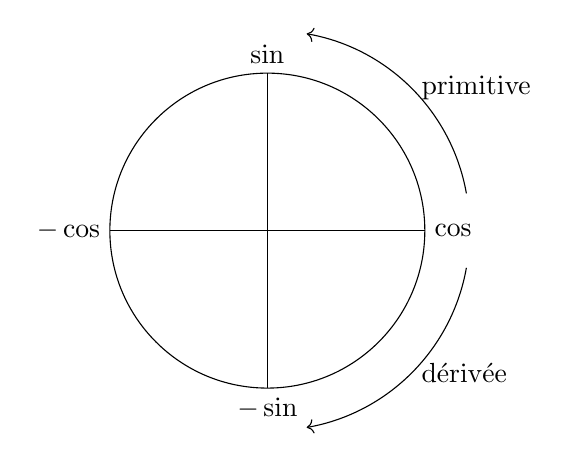
\begin{tikzpicture}
		\draw (0,0) -- (2,0) node[right] {$\cos$};
		\draw (0,0) -- (0,2) node[above] {$\sin$};
		\draw (0,0) -- (0,-2) node[below] {$-\sin$};
		\draw (0,0) -- (-2,0) node[left] {$-\cos$};
		\draw[<-] (0.5,2.5) arc (80:10:2.5) node[right, midway] {primitive};
		\draw[<-] (0.5,-2.5) arc (-80:-10:2.5) node[right, midway] {dérivée};
		\draw (0,0) circle (2);
	\end{tikzpicture}
	%\caption{Cercle des primitives et dérivées de sin et cos}
	\label{fig:cercle_primitives_derivees_sin_cos}
\end{figure}


\end{document}
